\documentclass{beamer}
\usepackage{outlines}
\usepackage{graphicx}
\graphicspath{{images/}}
\usetheme{CambridgeUS}
\usepackage{tikz}
\usepackage{pgfplots}
\pgfplotsset{compat=1.8}
\usepgfplotslibrary{statistics}
\usepackage{caption}
\usepackage{alltt}
\usepackage[utf8]{inputenc}

\title{Who is Chad Jenkins?}
\subtitle{Using Latex/Beamer}
\author{Chad Jenkins}
\institute{University of Nebraska}
\date{\today}

\begin{document}

\begin{frame}
\titlepage
\end{frame}

\begin{frame}
\frametitle{Who is Chad Jenkins?}
\begin{outline}
\1 Hi, my name is Chad Jenkins!
\2 Born May 2nd, 1989 in Lincoln, NE
\2 Husband of 9 yrs, father of 3
\2 Employed as Dairy Nutritionist
\2 Ph.D. candidate in Animal Science
\3 Anticipated graduation date: August 2022
\end{outline}
\end{frame}

\begin{frame}
\frametitle{Chad's Favorite Animal}

\includegraphics[scale=0.5]{animal}
\end{frame}

\begin{frame}
\frametitle{Chad's Favorite Plot}
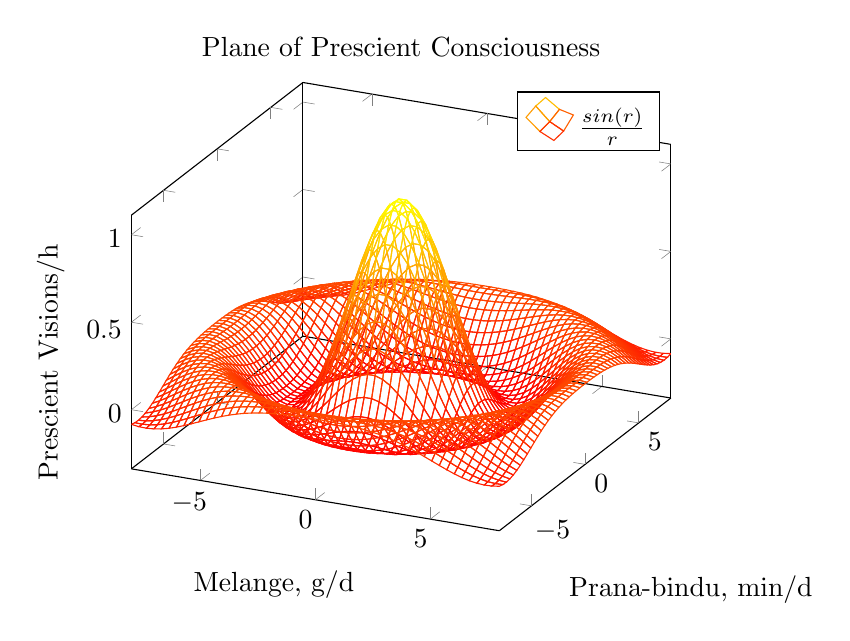
\begin{tikzpicture}
\begin{axis}[
    title=Plane of Prescient Consciousness,
    colormap/redyellow,
    xlabel={Melange, g/d},
    ylabel={Prana-bindu, min/d},
    zlabel={Prescient Visions/h}
]
\addplot3[
    mesh,
    samples=50,
    domain=-8:8,
]
{sin(deg(sqrt(x^2+y^2)))/sqrt(x^2+y^2)};
\addlegendentry{\(\frac{sin(r)}{r}\)}
\end{axis}
\end{tikzpicture}
\end{frame}

\begin{frame}
\frametitle{Link to Chad's CV}
\url{https://stat850-unl.github.io/11-presentation-chaddybox/jenkins_CV.pdf}
\end{frame}
\end{document}


